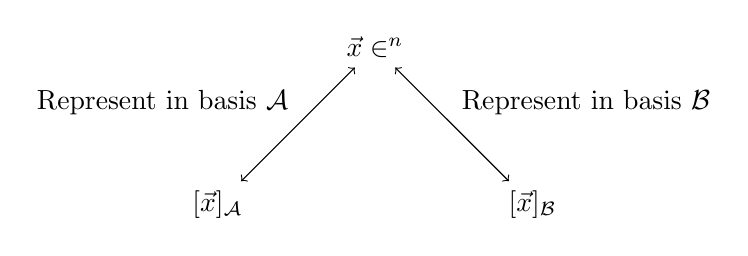
\begin{tikzpicture}
	\node (A) at (0,0) {$\vec x\in \R^n$};
	\node (B) at (-2,-2) {$[\vec x]_{\mathcal A}$};
	\node (C) at (2,-2) {$[\vec x]_{\mathcal B}$};
	\draw[<->] 
		(A) edge  node[midway, above left] {Represent in basis $\mathcal{A}$}(B)
		(A) edge  node[midway, above right] {Represent in basis $\mathcal{B}$} (C);
\end{tikzpicture}
